% SHAHID Phase 1 submission paper (IEEE conference format, A4).
% Build: python -m shahid.build_proposal --draft   (or --final; writes SHAHID_Phase1_Proposal.pdf)
\documentclass[conference,a4paper]{IEEEtran}

% ---- build mode: draft prints placeholders in red; final stops with a list of them ----
\newif\iffinal
\InputIfFileExists{buildmode.tex}{}{}  % written by shahid.build_proposal; absent = draft

\usepackage{fontspec}
\setmainfont{texgyretermes}[Extension=.otf, UprightFont=*-regular, BoldFont=*-bold,
  ItalicFont=*-italic, BoldItalicFont=*-bolditalic]
\setsansfont{texgyreheros}[Extension=.otf, UprightFont=*-regular, BoldFont=*-bold,
  ItalicFont=*-italic, BoldItalicFont=*-bolditalic]
\usepackage{unicode-math}
\setmathfont{texgyretermes-math.otf}

\usepackage{graphicx}
\usepackage{booktabs}
\usepackage{array}
\usepackage{tabularx}
\usepackage{xcolor}
\usepackage{tikz}
\usetikzlibrary{positioning, arrows.meta, fit, backgrounds, calc}
\usepackage{enumitem}
\setlist{leftmargin=1.1em, itemsep=0pt, topsep=1pt, parsep=0pt}
\usepackage{url}
\def\UrlBreaks{\do\/\do-\do.\do_\do=\do?\do\&}
\usepackage[hidelinks, pdftitle={SHAHID: Telling Power Outages from Lost Meter Data at the
  Distribution Transformer}, pdfauthor={Anonymous}, pdfsubject={}, pdfkeywords={},
  pdfcreator={}, pdfproducer={}]{hyperref}
\usepackage{cite}

\renewcommand{\arraystretch}{1.08}
\newcolumntype{L}[1]{>{\raggedright\arraybackslash}p{#1}}
\newcolumntype{Y}{>{\raggedright\arraybackslash}X}
\newcolumntype{Z}{>{\centering\arraybackslash}X}
\newcolumntype{C}[1]{>{\centering\arraybackslash}p{#1}}
\newcommand{\tabfont}{\footnotesize}

% ---- placeholders the team must fill (never filled by guesses) ----
\makeatletter
\newcount\teamtodocount
\gdef\teamtodolist{}
\newcommand{\teamtodo}[1]{%
  \ifcsname tt@\detokenize{#1}\endcsname\else
    \expandafter\gdef\csname tt@\detokenize{#1}\endcsname{}%
    \global\advance\teamtodocount by 1
    \xdef\teamtodolist{\teamtodolist^^J  [\the\teamtodocount] \detokenize{#1}}%
  \fi
  \textcolor{red}{[#1]}}
\AtEndDocument{%
  \iffinal\ifnum\teamtodocount>0
    \typeout{^^JUNFILLED PLACEHOLDERS (\the\teamtodocount):\teamtodolist^^J}%
    \errmessage{Final build stopped: \the\teamtodocount\space placeholder(s) still in the document; see the list above}%
  \fi\fi}
\makeatother

% ---- submission settings: edit here only ----
\newcommand{\authorline}{Anonymous submission}  % or: Team code: <code from the submission form>

\begin{document}

\title{SHAHID: Telling Power Outages from\\Lost Meter Data at the Distribution Transformer}
\author{\IEEEauthorblockN{\authorline}
\IEEEauthorblockA{IEEE TSYP14 EnergyMind Tunisia challenge, Phase 1}}
\maketitle

\begin{abstract}
SHAHID is a probabilistic artificial intelligence trust layer between smart-meter data and dispatch
decisions. When a group of meters under one distribution transformer stops reporting, it decides
whether the customers lost power or whether only their data stopped. A meter on the low-voltage side
of the transformer still sees the energy of customers whose data stopped, but not the energy of
customers who lost power. SHAHID compares that unexplained energy with the consumption it expects
from the silent customers, scores both causes with heavy-tailed likelihoods, and decides only when
the evidence is decisive; otherwise it abstains and hands the case to a person with the evidence, a
plain-language explanation and a tamper-evident log entry. All evidence is simulated on public German
benchmark networks. With thresholds frozen on one network and each evaluation run once, the method
called no labelled communication failure an outage on four other networks, missed at most one outage
in a hundred, and decided about half to three quarters of the events. On data with no events, random
single-meter data losses still produced about 15 to 33 false outage verdicts per transformer-year under the
registered configuration; a post-hoc gate reduced this to 0.2 to 1.0. The evaluations also measure
where the method fails: small silent groups, unmetered energy that follows the load, simultaneous
events and hourly readings. The method requires an energy meter at each transformer and does not
detect faults inside a single meter.
\end{abstract}

\begin{IEEEkeywords}
abstention, advanced metering infrastructure, communication failure, distribution networks, energy
balance, explainability, human oversight, outage detection, selective prediction, smart meters
\end{IEEEkeywords}

\section{Introduction}\label{sec:intro}
The Tunisian utility, the Société Tunisienne de l'Électricité et du Gaz (STEG), is deploying smart
meters. Press reports of a STEG briefing put the count at about 80,000 low-voltage (LV) meters in
pilot zones by the end of March 2026, with a first phase of 450,000 electricity meters
\cite{africanmanager2026compteurs,webdo2026compteurs}. STEG serves about 4.7 million subscribers,
most of them residential LV customers \cite{lapresse2025steg}. In the summer of 2026 the same network
went through rotating power cuts during a heatwave
\cite{newarab2026heatwave,africanmanager2026heat,webdo2026delestages}. These facts come from
secondary sources; they motivate the problem and enter no result.

As this advanced metering infrastructure (AMI) grows, operators will see groups of meters go silent.
From the meter data alone they cannot tell an \emph{outage}, which needs a crew, from a
\emph{communication failure}, which does not. A wrong call either wastes a truck roll or leaves
customers without power and unattended. SHAHID addresses this one question for one LV neighbourhood
under one medium-voltage/low-voltage (MV/LV) transformer, with 15-min readings. It is a probabilistic
artificial intelligence (AI) trust layer between smart-meter data and dispatch decisions.

\textbf{Hypothesis.} A meter on the LV side of the transformer still measures the energy of customers
whose data stopped, and no longer measures the energy of customers who lost power. If this difference
is large compared with the uncertainty of the expected consumption, the two causes can be separated.

\textbf{Contributions.} All results are SIMULATED.
\begin{enumerate}[leftmargin=1.4em]
\item A transformer-side energy-balance test with abstention that, with thresholds frozen on one
network, called no labelled communication failure an outage in every registered evaluation, on four
networks never used for tuning. On data with no events, random single-meter data losses still produced
about 15 to 33 false outage verdicts per transformer-year under the registered configuration; a post-hoc
gate reduced this to 0.2 to 1.0 (Section~\ref{sec:results}).
\item A measured operating envelope: the resolution limit, the reporting interval, and five conditions
under which the method weakens or fails (Section~\ref{sec:weakens}).
\item Governance measured, not assumed: an escalation table whose automatic rule was found to close
real outages and was made provisional, operator load per transformer-day, a hash-chained decision log
and an operator console preview (Sections~\ref{sec:explain}--\ref{sec:governance}).
\item A failure mechanism measured and removed: a powered meter merged into an outage group can
explain the whole residual; splitting silent groups by feeder removed the confident wrong verdicts it
caused, 4 to 0 (Section~\ref{sec:phase2}).
\item A verifiable evidence chain: protocols committed before each confirmatory run, negative results
reported, and every number in this paper checked by code against a claims ledger
(Section~\ref{sec:protocol}).
\end{enumerate}

\section{Related Work}\label{sec:related}
\textbf{Outages from AMI messages.} Meters with outage notification send a ``last gasp'' message when
power is lost, and utilities can ``ping'' meters to bound an outage \cite{doe2016ami}; pinging is also
used to monitor grid-edge devices \cite{huang2021pinging}, and pings can enter a joint estimate of
topology and outages \cite{gandluru2019joint}. SHAHID uses neither: its decision rests on interval
energy alone, for the case where messages are absent or unreliable.

\textbf{Outages from flows and forecasts.} Sevlian et al.\ detect outages by combining line-flow
measurements with load forecasts at the nodes of a distribution tree \cite{sevlian2015outage}; Wang et
al.\ learn the normal distribution of smart-meter data per region \cite{wang2024outage}; a review
surveys smart-meter analytics \cite{wang2018review}. SHAHID shares the principle of comparing a
measured upstream flow with a forecast of downstream consumption, and applies it to a narrower
question: which cause explains a group of meters that stopped reporting.

\textbf{Deciding with a reject option.} Chow characterised the trade-off between error and reject
\cite{chow1970reject}; selective classification trades coverage for accuracy
\cite{elyaniv2010selective,geifman2017selective}, and reject strategies are compared in
\cite{franc2023reject}. SHAHID's threshold rule is a constrained selection of this kind: it bounds
missed and false outages, then maximises coverage. We make no novelty claim; these comparisons
position the work.

\section{Scope and Objectives}\label{sec:scope}
\textbf{Scope.} One LV neighbourhood under one MV/LV transformer, about 100 customers. Inputs:
15-min energy per customer meter with its arrival time, 15-min energy from one meter on the
transformer's LV side, and static context (which meters share a line section or a data concentrator,
installed photovoltaic (PV) power per customer). Output per silent group: OUTAGE, COMMUNICATION
FAILURE or UNCERTAIN, with a probability, an explanation and a log entry.

\textbf{Non-goals in Phase 1.} No real data, no hardware, no deployed or real-time operation, no
control action on the grid, no claim that the data represents Tunisia. Faults inside a single meter
are tested but outside the validated scope (Section~\ref{sec:singlemeter}). Current and power quality
are out of scope: 15-min energy readings carry no waveform quantities.

\textbf{Objectives, mapped to the brief.}
\begin{itemize}
\item \textbf{G1, anomaly detection:} tell a genuine grid event from a data problem for silent groups;
measure where this stops working (Sections~\ref{sec:method}, \ref{sec:results}).
\item \textbf{G2, confidence and explanation:} a probability, a plain-language explanation and an
auditable record for every verdict (Section~\ref{sec:explain}).
\item \textbf{G3, escalation and governance:} rules for what the system may do alone, measured
against their harm and their operator load (Section~\ref{sec:governance}).
\item \textbf{G4, shared learning across nodes:} what is shared, what stays local and why, with a
measured proof of concept (Section~\ref{sec:shared}).
\end{itemize}
Appendix~\ref{app:coverage} maps every item of the brief to its status and evidence.

\section{Data and Anomaly Simulation}\label{sec:data}
No STEG data is available to us, and no public dataset combines customer meter readings, a transformer
meter, a communication layer and labelled causes. We therefore simulate the network and its
measurement chain and label every event where it is injected. Table~\ref{tab:data} states what is real
and what is simulated, class by class.

\begin{table*}[!t]
\caption{What is real and what is simulated, class by class}\label{tab:data}
\centering\tabfont\setlength{\tabcolsep}{3.5pt}
\begin{tabularx}{\textwidth}{@{}L{0.21\textwidth} L{0.09\textwidth} Y L{0.21\textwidth}@{}}
\toprule
\textbf{Element or anomaly class} & \textbf{Layer} & \textbf{Generation rule} & \textbf{Status (default value)} \\
\midrule
Networks, load and PV profiles & truth & Public German benchmark LV networks with their 2016 profiles (SimBench) \cite{meinecke2020simbench} & REUSED, real benchmark data, not Tunisian \\
Electrical state & truth & AC power flow at every 15-min step (pandapower) \cite{thurner2018pandapower} & REUSED solver \\
Customer diversity & truth & Per-customer daily shift, daily scale and correlated noise around the benchmark shapes, one parameter $d$ & ASSUMPTION, results over its range \\
Physical outage & truth & A line is opened and the power flow is re-solved; isolated customers and their PV drop to zero & SIMULATED, from the event file \\
Real load change & truth & The load of a set of customers is scaled, then re-solved & SIMULATED, factor 0.3 to 2.5 \\
Unmetered energy & truth & Added to the transformer series, constant or following the load shape & SIMULATED, none by default \\
Communication failure & observation & Readings of a concentrator, line section or random set stop; stored readings arrive after the link returns & SIMULATED, late delivery on \\
Random missing reading & observation & Each reading is lost independently & ASSUMPTION, probability 0.01 \\
Delayed reading & observation & Each reading may arrive some intervals late & ASSUMPTION, probability 0.03 \\
Meter and transformer-meter error & observation & Fixed gain, noise and quantisation per device & ASSUMPTION, gain sd 0.005 and 0.002 \\
Single-meter faults (study only) & observation & Gain, bias and noise injected into one meter for seven days & SIMULATED, not in the dataset \\
Power-loss (last-gasp) message & observation & Optional message at outage onset & implemented, off in every result \\
\bottomrule
\end{tabularx}
\end{table*}

The simulator writes four separate stores: hidden physical truth, the observed data a utility export
could contain, static context, and labels. The detector reads only observed data and context; a test
fails if it opens truth or labels. Outages and communication failures are drawn from the same sets of
customers, so the pattern of silent meters carries no information about the cause. Every generator
parameter is a configuration value in the repository, and the committed dataset regenerates with one
command per folder.

\section{Detection Method (G1)}\label{sec:method}
Fig.~\ref{fig:pipeline} shows the pipeline. Meters whose readings for two consecutive intervals have
not arrived form a \emph{silent group} with a common onset $t_0$. At a decision time $\tau$, using only
data that had arrived by $\tau$, the method computes over the window $w=[t_0,\tau)$
\begin{align}
R &= \textstyle\sum_{t\in w}\big(T_t - \sum_{m\in K_t} E_{m,t} - g_0 - \hat{O}_t\big), \label{eq:R}\\
M &= \textstyle\sum_{t\in w}\sum_{m\in G}\big(\bar{E}_{m,t} + \rho_{\ell}\,\delta_{m}\big), \label{eq:M}
\end{align}
where $T_t$ is the transformer's LV energy in interval $t$, $K_t$ the meters whose reading for $t$
has arrived, $E_{m,t}$ their energy, $g_0$ the median transformer-to-meters gap over the last day,
$\hat{O}_t$ the expected energy of other missing meters, $G$ the silent group, $\bar{E}_{m,t}$ the mean
of the same 15-min slot over the previous 14 days, $\delta_m$ the deviation of meter $m$ from that
mean just before the onset, and $\rho_\ell$ a persistence factor fitted per lead $\ell$. All energies
are in kWh. If the customers still have power, $R \approx M$; if they lost it, $R \approx 0$.

\begin{figure*}[!t]
\centering
% System pipeline (illustration). Every element is named in the paper text (Sections V to VIII).
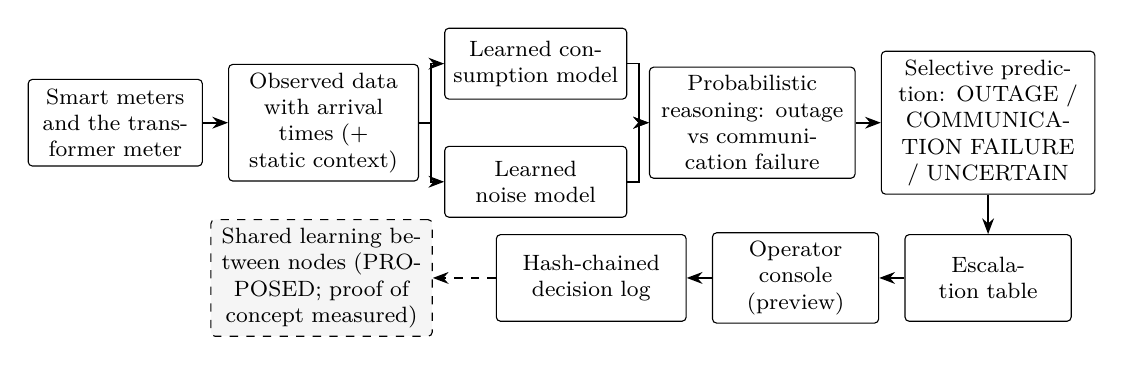
\begin{tikzpicture}[
  font=\footnotesize, node distance=4mm and 3.2mm,
  box/.style={draw, rounded corners=1.5pt, align=center, inner sep=3pt, minimum height=11mm, text width=#1},
  box/.default=21mm,
  prop/.style={box=#1, dashed, fill=gray!8},
  prop/.default=21mm,
  arr/.style={-{Stealth[length=2mm]}, semithick}]
\node[box=20mm] (meters) {Smart meters and the transformer meter};
\node[box=22mm, right=of meters] (obs) {Observed data with arrival times (+ static context)};
\node[box=21mm, right=of obs, yshift=7.5mm, minimum height=9mm] (cons) {Learned consumption model};
\node[box=21mm, right=of obs, yshift=-7.5mm, minimum height=9mm] (noise) {Learned noise model};
\node[box=24mm, right=of obs, xshift=26mm] (reason) {Probabilistic reasoning: outage vs communication failure};
\node[box=25mm, right=of reason] (sel) {Selective prediction: OUTAGE / COMMUNICATION FAILURE / UNCERTAIN};
\node[box=19mm, below=5mm of sel] (esc) {Escalation table};
\node[box=19mm, left=of esc] (op) {Operator console (preview)};
\node[box=22mm, left=of op] (log) {Hash-chained decision log};
\node[prop=26mm, left=8mm of log] (share) {Shared learning between nodes (PROPOSED; proof of concept measured)};
\draw[arr] (meters) -- (obs);
\draw[arr] (obs.east) -- ++(1.5mm,0) |- (cons.west);
\draw[arr] (obs.east) -- ++(1.5mm,0) |- (noise.west);
\draw[arr] (cons.east) -- ++(1.5mm,0) |- (reason.west);
\draw[arr] (noise.east) -- ++(1.5mm,0) |- (reason.west);
\draw[arr] (reason) -- (sel);
\draw[arr] (sel) -- (esc);
\draw[arr] (esc) -- (op);
\draw[arr] (op) -- (log);
\draw[arr, dashed] (log) -- (share);  % confirmed outcomes with their evidence numbers (Section 5.4)
\end{tikzpicture}

\caption{System pipeline. Solid boxes are IMPLEMENTED and evaluated in simulation; dashed boxes are
PROPOSED. The meter-count gate and the re-check of Section~\ref{sec:governance} are evaluated in study
code and are not yet executed by the escalation step.}\label{fig:pipeline}
\end{figure*}

\textbf{Decision.} With Student-t likelihoods of 4 degrees of freedom, scales $s_O$ (outage) and
$s_C$ (communication failure) built from the fitted gap noise and forecast spread, and a prior of
one half for each cause, the posterior probability of a communication failure is
\begin{equation}
p = \sigma\!\left(\ln f_\nu\!\left(\tfrac{R-M}{s_C}\right) - \ln s_C - \ln f_\nu\!\left(\tfrac{R}{s_O}\right) + \ln s_O\right), \label{eq:p}
\end{equation}
where $f_\nu$ is the Student-t density and $\sigma$ the logistic function. The verdict is
COMMUNICATION FAILURE if $p \ge 1-b$, OUTAGE if $p \le b$, and UNCERTAIN otherwise, with abstention
band $b = 0.03$. The decision is taken at the first of up to five decision times at which it is not
UNCERTAIN.

\textbf{Fitting and threshold selection.} Noise and persistence parameters are fitted on each
network's own fault-free history (training weeks); no labelled data is needed. The band $b$ was chosen
once, on development validation weeks, as the setting that abstains least while keeping missed
outages at or below 0.05, false outages at or below 0.05 and fault-free false outages at or below
0.001 per meter-day (DESIGN CHOICE). Two earlier selection rules failed and are reported in the
repository: one called 419 of 1051 fault-free silent groups outages, the other missed 0.366 of outages.

\textbf{Why not a trained classifier.} Under the same safety limits, logistic regression, gradient
boosting and a small neural network trained on simulated labels missed 0.089, 0.179--0.196 and
0.232--0.250 of validation outages, against 0.036 for the fitted method; none had a feasible
abstention band (Fig.~\ref{fig:classifiers}). The fitted probabilistic parameters are therefore the
trained models of this submission, by a measured choice.

\begin{figure}[!t]
\centering
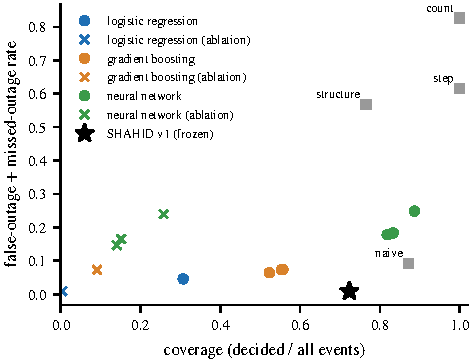
\includegraphics[width=\columnwidth]{figures/classifier_coverage_safety.pdf}
\caption{Coverage against false-outage plus missed-outage rate on the held-out urban network, test
weeks (SIMULATED, post-hoc). Dots: classifiers, one per seed; crosses: without energy-balance
features; squares: simple baselines; star: the frozen method.}\label{fig:classifiers}
\end{figure}

\subsection{Scope boundary: single-meter anomalies}\label{sec:singlemeter}
Silent groups were chosen first because the same symptom needs opposite responses and the
transformer gives an independent physical witness. Faults inside one meter that keeps reporting
(gain, bias, noise) are a different problem: the balance can show that some meter is
wrong, not which one. We tested them. Injected gain errors, biases and noise on one meter were
detected in at most 20\% of cases; a per-meter regression of the transformer gap detected a gain of
0.5 in 0.347 of cases on a network never used before, and neighbour-voltage comparison detected at
most 0.053. Single-meter fault detection is therefore outside the validated scope. The Phase 2 path
(PROPOSED, not implemented): residual drift tracked per meter over weeks, comparison with electrically
adjacent meters with field voltage data, and escalation to human review instead of automatic action.

\section{Confidence, Explanation and Audit (G2)}\label{sec:explain}
\textbf{Confidence score.} Every verdict carries the posterior $p$ of (\ref{eq:p}). On the held-out
network, probabilities below 0.1 (80 events) and above 0.9 (124 events) match the observed shares of
communication failures (0.013 and 0.992). Over all 6210 held-out silent groups, mid-range values are
not calibrated frequencies (expected calibration error 0.494), because most small groups are data
losses decided under an equal prior. The console therefore labels mid-range values ``current evidence
strength, not validated accuracy''.

\textbf{Plain-language explanation.} A fixed template is filled from the verdict record: how many
meters went silent and when, the expected energy $M$, the unexplained energy $R$ with the spread
expected under each cause, the probability, the alternative cause and, when abstaining, the reason. A
test fails if an explanation contains a number that is not in the record. Templates, not generated
text, were chosen so that no explanation can state a number the system did not compute. The decision
is interpretable by construction: it rests on two physical quantities in kWh, $R$ and $M$, that an
operator can check against the transformer reading; post-hoc explainers such as SHAP
\cite{lundberg2017shap} were used only to inspect the comparison classifiers. Whether
people can act on the explanations alone is registered as a study (protocol 07b) whose results are
pending.

\textbf{Auditable log.} Each record (evidence, verdict, explanation, escalation rule) is appended to an
append-only text log, one record per line; each entry stores the SHA-256 hash of the previous one, so any edit or deletion breaks
the chain, and a test checks that a single edit is detected. Operator actions in the console go into
a second chain of the same kind. The record answers what was detected, what was concluded and why.

\section{Escalation and Governance (G3)}\label{sec:governance}
\textbf{Thresholds for automatic action.} Table~\ref{tab:escalation} is the escalation table, a
configuration file (DESIGN CHOICE, not validated with operators). The only action taken without a
person annotates data and opens a ticket; dispatching a crew or contacting customers always needs a
person. As first written, rule R3 closed communication verdicts automatically. Measured on simulated
events, it closed real outages without supervision in 0.9\% to 1.8\% of cases nominally and in
24.1\% under 10 kW of load-shaped unmetered energy, so it was made provisional with a re-check.

\begin{table}[!t]
\caption{Escalation table (first matching rule wins)}\label{tab:escalation}
\centering\tabfont\setlength{\tabcolsep}{3pt}
\begin{tabularx}{\columnwidth}{@{}l Y L{0.20\columnwidth}@{}}
\toprule
\textbf{Rule} & \textbf{Condition and action} & \textbf{Handled by} \\
\midrule
R1 & Outage verdict on 20 meters or more: alert at once; operator decides on dispatch & human \\
R2 & Outage verdict with probability 0.95 or more: alert with the evidence; operator confirms & human \\
R3 & Communication verdict, probability 0.95 or more, at most 40 meters: provisional data-quality ticket; re-check the backlog of readings & automatic, provisional \\
R4 & Any other communication verdict: ticket reviewed within the shift & human \\
R5 & Abstention: review with the evidence & human \\
\bottomrule
\end{tabularx}
\end{table}

\textbf{Operator load.} With 1\% of readings lost at random and no events, version 1 sends 10.23 items
per transformer-day to a person on the development network, almost all one- or two-meter silences.
A meter-count gate (post-hoc variant) watches groups of fewer than 3 meters for one hour. On a network
never used before, the gate that escalates instead of closing cut human items from 9.80 to 4.15 per
transformer-day and false outage verdicts from 15.0 to 0.5 per transformer-year, with no outage
closed silently among 350 whole-feeder outages. The gate that closes lost 16 of 350 outages on
development data. \textbf{Implementation status:} the gate and the R3 re-check are evaluated in study
code; neither is yet executed by the escalation step.

\textbf{Operator interface.} A validation and audit console (IMPLEMENTED as a preview, Streamlit)
replays stored simulated days through the frozen pipeline: three queues that are never merged (outage
awaiting approval, uncertain case, unconfirmed communication verdict), an evidence card per item with
the alternative cause, a network map, and the hash-chained operator log with chain verification.
Replay comes before live operation by design: verdicts and thresholds can be checked against known
outcomes first. No operator has used it.

\textbf{Over-trust and under-trust.} Against over-trust: the alternative cause is shown with every
verdict, a random sample of automatic closures goes to audit,
and approvals given within seconds are flagged. Against under-trust: a track record per verdict class
and overrides recorded with their outcome. These devices are implemented in the console; their effect
on operators is not measured.

\section{Shared Learning Across the Noosphere (G4)}\label{sec:shared}
\textbf{What is shared, what stays local, and why.} Shared between nodes: dimensionless fitted noise
parameters, frozen decision thresholds, each site's measured resolution limit, and (PROPOSED)
anonymous failure signatures such as ``the gap follows the load'' and operator-confirmed outcomes
stripped of identifiers. Kept local: every meter reading, customer and meter identifiers and network
topology, because interval consumption is personal data (DESIGN CHOICE).

\textbf{What was tested.} In a proof of concept, a new node received another node's noise-shape
parameters and fitted only its scale from $d$ days of its own data. The gain was negligible: with one
day of local data, the nominal interval covered 0.978 of fault-free residuals when fitted locally and
0.96 with shared parameters, and shared parameters gave more fault-free outage verdicts (9 against 4).
Local calibration is fast, so sharing noise parameters is the wrong mechanism.

\textbf{What did transfer.} Thresholds frozen on one network kept the false-outage rate at 0.0 on labelled communication failures on the
networks never used for tuning (Section~\ref{sec:results}). The design (PROPOSED) therefore rests on a
bulletin of frozen thresholds and anonymous failure signatures: a new node preloads them, abstention
rules are only ever tightened by shared knowledge, and no raw data leaves a site. A coordinator that
sees several neighbourhoods go silent at the same moment could also treat them as one upstream event,
such as a rotating cut.

\section{Evaluation Protocol}\label{sec:protocol}
\textbf{Networks and splits.} Thresholds were chosen on one semi-urban development network (104
customers). Each network is split by week into training, validation and test weeks. A held-out urban
network (111 customers) was evaluated once after the method and thresholds were frozen and the
protocol committed; an untouched rural network (118 customers) once later; and two networks never
used before (rural, 99 customers; semi-urban, 41 customers) once in a confirmatory batch
whose protocol was committed before the run. Events occur about once per day, an artificial rate
chosen to obtain enough events, not a field frequency.

\textbf{Metrics in the brief's terms.}
\begin{itemize}
\item \emph{Recall:} outage recall and communication recall, the share of each cause called correctly.
\item \emph{False-positive rate:} the false-outage rate (communication failures called outages), and
false outage verdicts per meter-day on fault-free data.
\item \emph{Missed detections:} the missed-outage rate (outages called communication failures or never
detected).
\item \emph{Coverage:} the share of events that receive a verdict. Accuracy when deciding is never
reported without it.
\item \emph{Latency:} intervals from silence to verdict. \emph{Explanation quality:} faithfulness by
test; usefulness by a registered people study (pending).
\end{itemize}
A labelled event matches a silent group with the same onset and a meter-set overlap (Jaccard index)
of at least 0.5; otherwise it is missed.

\textbf{Integrity.} Every number in this paper has a row in a claims ledger naming its result file,
command, commit and configuration hash; a checker compares the paper with the ledger and the result
files, and every table number must appear verbatim in a generated results document. The checker
cannot catch a wrong two-decimal rate between 0 and 1, and we say so.

% Sources (checked by shahid.check_numbers): results/cp7_heldout.json results/iforest.json
% results/leak_audit.json results/cp12.json results/p2/confirm.json; ledger C7-01, AU-01, CP12-T5, P2C-01..05, CAD-1..4, TN-H1..H4
\section{Results}\label{sec:results}
All results are SIMULATED.

\subsection{Held-out network and baselines}\label{sec:heldout}
Table~\ref{tab:heldout} compares methods on identical observed inputs: 109 outages and 155
communication failures on the held-out network, test weeks, evaluated once.

\begin{table*}[!t]
\caption{Held-out urban network, test weeks, evaluated once}\label{tab:heldout}
\centering\tabfont
\begin{tabularx}{\textwidth}{@{}L{0.25\textwidth}ZZZZZZZ@{}}
\toprule
\textbf{Method} & \textbf{Coverage} & \textbf{Accuracy when deciding} & \textbf{Outage recall} & \textbf{Comms recall} & \textbf{False outage} & \textbf{Missed outage} & \textbf{Fault-free false outages per meter-day} \\
\midrule
SHAHID version 1 (with abstention) & 0.723 & 0.995 & 0.670 & 0.755 & 0.000 & 0.009 & 0.0010 \\
Two-sided z-test$^{a}$ & 0.636 & 0.994 & 0.615 & 0.645 & 0.000 & 0.009 & 0.0002 \\
Likelihood ratio without abstention$^{a}$ & 0.720 & 0.963 & 0.716 & 0.677 & 0.039 & 0.009 & 0.0038 \\
Visible-share test$^{a}$ & 0.720 & 0.963 & 0.725 & 0.671 & 0.045 & 0.000 & 0.0045 \\
Naive share baseline$^{b}$ & 0.871 & 0.943 & 0.890 & 0.774 & 0.065 & 0.028 & 0.0104 \\
Step baseline (transformer drop) & 1.000 & 0.682 & 0.752 & 0.632 & 0.368 & 0.248 & 0.0629 \\
Count baseline (share of section silent) & 1.000 & 0.545 & 0.826 & 0.348 & 0.652 & 0.174 & 0.0039 \\
Structure baseline (silence pattern)$^{b}$ & 0.765 & 0.604 & 0.624 & 0.348 & 0.394 & 0.174 & 0.0031 \\
Isolation Forest \cite{liu2008isolation} (added afterwards) & 1.000 & 0.447 & 0.972 & 0.077 & 0.923 & 0.028 & 0.0057 \\
\bottomrule
\multicolumn{8}{@{}p{\textwidth}@{}}{\scriptsize $^{a}$Coverage below 1 without an abstention band: these methods answer UNCERTAIN when the expected energy of the silent group is below a minimum chosen on validation weeks; the z-test also when both or neither cause fits. $^{b}$The naive baseline has its own minimum-energy rule; the structure baseline abstains when the silent set is both a concentrator group and a line section. The count and step baselines and the Isolation Forest never abstain.}
\end{tabularx}
\end{table*}

Version 1 is the safest method, not the one that decides most often: the naive baseline decides
0.871 of events but calls 0.065 of communication failures outages. On development validation data,
only version 1 (coverage 0.663) and the z-test (0.602) can meet the three safety limits at any
setting. The Isolation Forest detects that something happened but cannot attribute the cause (AUC
0.41, 95\% interval 0.341--0.484, where AUC is the area under the receiver operating characteristic curve).
\textbf{Leak check:} replacing the transformer series with a copy shifted by seven days drops outage
recall from 0.641 to 0.103; the decisions depend on the transformer signal.

\subsection{Every frozen evaluation}\label{sec:allgrids}
Table~\ref{tab:allgrids} lists every evaluation of the frozen method. The development row uses unseen
weeks of the network on which thresholds were chosen, so it is not held-out data.

\begin{table}[!t]
\caption{Every evaluation of frozen version 1 (95\% Wilson intervals where computed)}\label{tab:allgrids}
\centering\scriptsize\setlength{\tabcolsep}{2pt}
\begin{tabularx}{\columnwidth}{@{}Y C{0.21\columnwidth} C{0.21\columnwidth} C{0.21\columnwidth}@{}}
\toprule
\textbf{Network (run)} & \textbf{Coverage} & \textbf{False outage} & \textbf{Missed outage} \\
\midrule
Development, test weeks & 0.697 (0.639--0.749) & 0.000 (0.000--0.024) & 0.000 (0.000--0.035) \\
Held-out urban (once) & 0.723 (0.667--0.774) & 0.000 (0.000--0.024) & 0.009 (0.002--0.050) \\
Untouched rural (once) & 0.494 (0.421--0.568) & 0.000 (0.000--0.034) & 0.000 (0.000--0.055) \\
Never used, rural, 99 meters (once) & 0.670 (---)$^{a}$ & 0.000 (---)$^{a}$ & 0.009 (---)$^{a}$ \\
Never used, semi-urban, 41 meters (once) & 0.527 (---)$^{a}$ & 0.000 (---)$^{a}$ & 0.000 (---)$^{a}$ \\
\bottomrule
\multicolumn{4}{@{}p{\columnwidth}@{}}{\scriptsize $^{a}$Wilson interval not computed for the confirmatory runs.}
\end{tabularx}
\end{table}

Accuracy when deciding was 1.0 on both never-used networks. The false-outage rates of
Table~\ref{tab:allgrids} (0.000) concern labelled communication failures. On fault-free data the two
never-used networks gave 0.0004 and 0.0006 false outages per meter-day. On data with no events,
random single-meter data losses still produced about 15 to 33 false outage verdicts per
transformer-year under the registered configuration; a post-hoc gate reduced this to 0.2 to 1.0
(Section~\ref{sec:governance}). Across the first three evaluations, outage recall was 0.42--0.67 and
communication recall 0.54--0.75. The median decision latency is 2 intervals after the meters go
silent.

\subsection{Resolution limit and where the method weakens}\label{sec:weakens}
The method is correct with probability 0.90 once the expected silent energy is about 6 times its
predictive uncertainty: a signal-to-noise ratio (SNR) of 6.1 (5.2--7.3) on the development network
and 4.9 (4.2--5.6) on the held-out network (Fig.~\ref{fig:snr}). A single silent customer is below
this limit, so it usually receives an abstention; the rare wrong verdicts on one- and two-meter groups
are the fault-free false outages of Section~\ref{sec:governance}.

\begin{figure}[!t]
\centering
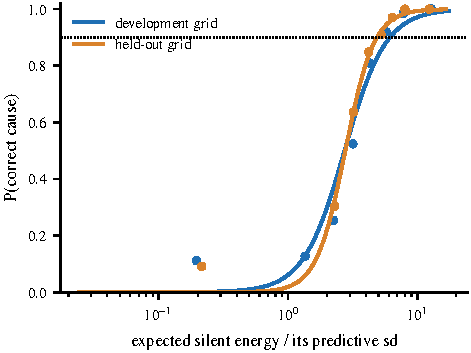
\includegraphics[width=\columnwidth]{figures/snr_detectability.pdf}
\caption{Probability of a correct verdict against the ratio of expected silent energy to its
uncertainty (SIMULATED; dots are binned shares, lines are logistic fits; dotted line at
0.9).}\label{fig:snr}
\end{figure}

Table~\ref{tab:weakens} lists the conditions that degrade the method, on the development network with
frozen thresholds, and the reporting-interval sensitivity on three networks with new seeds
(post-hoc).

\begin{table}[!t]
\caption{Conditions under which version 1 weakens or fails}\label{tab:weakens}
\centering\scriptsize\setlength{\tabcolsep}{2.5pt}
\begin{tabularx}{\columnwidth}{@{}Y C{0.14\columnwidth} C{0.14\columnwidth} C{0.14\columnwidth}@{}}
\toprule
\textbf{Condition} & \textbf{Coverage} & \textbf{False outage} & \textbf{Missed outage} \\
\midrule
Transformer-meter gain error, sd 2\% & 0.567 & 0.019 & 0.046 \\
Load-shaped unmetered energy, 5 kW & 0.534 & 0.034 & 0.122 \\
Load-shaped unmetered energy, 10 kW & 0.538 & 0.045 & 0.241 \\
Outage and communication failure at once & 0.761 & 0.016 & 0.373 \\
10\% of readings lost at random & 0.490 & 0.000 & 0.135 \\
Midday with doubled PV & 0.528 & 0.000 & 0.013 \\
\midrule
Readings every 15 min (three networks) & 0.629 & 0.002 & 0.006 \\
Readings every 30 min & 0.555 & 0.012 & 0.036 \\
Readings every 60 min & 0.421 & 0.021 & 0.245 \\
\bottomrule
\end{tabularx}
\end{table}

\begin{itemize}
\item \textbf{Main weakness.} The method treats the normal gap as constant; unmetered energy that
follows the load and transformer-meter gain error both scale with load (Fig.~\ref{fig:unmetered}).
\item \textbf{Simultaneous events} merge into one silent group that looks like a communication failure.
\item \textbf{Reporting interval.} Quarter-hour readings are safe; half-hour readings are
inconclusive (missed outages 0.036, upper bound 0.052); hourly readings are outside the envelope,
mostly because short events no longer suppress two readings.
\item \textbf{Not sensitive to} constant unmetered energy, meter noise up to three times nominal,
history length, PV share or concentrator layout. Coverage spans 0.484 to 0.663 over the range of the
uncalibrated diversity parameter.
\end{itemize}

\begin{figure}[!t]
\centering
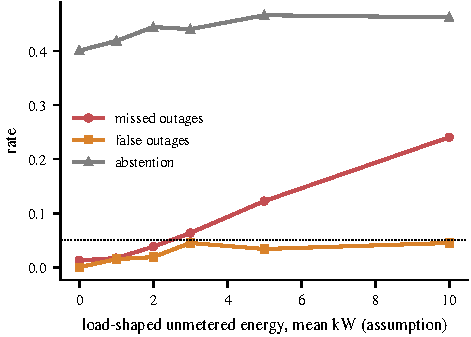
\includegraphics[width=\columnwidth]{figures/unmetered_failure.pdf}
\caption{Missed and false outages, and abstention, as load-shaped unmetered energy increases
(SIMULATED, development network; dotted line at the 5\% limit).}\label{fig:unmetered}
\end{figure}

\subsection{Further studies (protocols committed before running)}\label{sec:phase2}
\begin{itemize}
\item \textbf{Merged powered meter.} A powered meter that goes silent at the same moment as an outage
can join the outage group and supply its residual; on whole-feeder runs of the never-used rural network this happens
15.0 times per transformer-year. This is a different quantity from the 15.0 false outage verdicts
of Section~\ref{sec:governance}: both count 30 events over the same exposure, but in separate
simulations (whole-feeder outages here, fault-free data there). Splitting silent groups by feeder removed every confident wrong verdict it
caused (4 to 0) and stayed within the safety limits, at a price: abstention on random-meter
communication failures rose from 0.405 to 0.973.
\item \textbf{Negative results.} A prior that depends on group size missed 0.107 to 0.321 of
outages, above the limit; evidence accounting version 2 missed more mid-interval outages than version 1
(0.257 against 0.117). Version 1 stays the registered method.
\end{itemize}

\subsection{Deployment modes (Tunisia study)}\label{sec:tunisia}
A further study, on the same simulated networks with new seeds, varied the unknown Tunisian deployment
conditions; every value is an ASSUMPTION. Frozen version 1 transferred in 15 of 24 families and failed
under 10\% random loss and load-shaped unmetered energy. A transformer series delayed by a day costs
only time. Without a transformer measurement, every energy-balance method answers UNSUPPORTED for
0.997 of episodes: the transformer meter is a prerequisite, not an option. With daily batch delivery
the diagnosis becomes retrospective (median delay 10.25 h).

% Sources (checked by shahid.check_numbers): results/business/business.json (its stamp holds
% configs/business.yaml); ledger BUS-01..05, P2C-04, P2D-02
\section{Deployment and Business Case}\label{sec:business}
All money is in Tunisian dinars (TND). No price was invented: a unit cost without a public source is
shown as a formula (Table~\ref{tab:cost}). The full case and its parameters are in the repository
(\texttt{docs/BUSINESS\_CASE.md}, \texttt{configs/business.yaml}).

\textbf{Prerequisites.} An LV energy meter at each transformer, read every 15 min, is required; it is a
costed hardware line wherever absent. A head-end export of readings with arrival times, the line and
zone register from the geographic information system (GIS), and the concentrator mapping complete the
inputs.

\textbf{Implementation.} One pilot district the size of the STEG agency of Douz: about 24,400
customers and 149 transformer substations \cite{managers2026douz}. Phase A replays 90 days of the
district's history with fits per transformer; Phase B runs in shadow. Go/no-go uses the frozen safety
limits (missed and false outages at most 0.05, fault-free false outages at most 0.001 per meter-day);
coverage and operator load are reported for STEG to judge.

\textbf{Production and data protection.} Decision and operator logs are append-only and hash-chained;
crew dispatch always needs a person. Readings stay inside the utility. Organic Law 2004-63 applies,
and a draft organic law of 132 articles, heard in parliament in February 2026, names data processing
by artificial intelligence \cite{businessnews2026loi}.

\textbf{Continuous training.} No labels are needed: each transformer's parameters are refitted on its
own fault-free data every 90 days and after any topology change (DESIGN CHOICE); thresholds stay
frozen. The fault-free false-outage rate per meter-day is the drift indicator.

\textbf{Integration.} Inputs from the AMI head-end, the transformer meter and the GIS; outputs to the
outage-management or ticketing system and to the audit store.

\begin{table*}[!t]
\caption{Deployment cost for a district of 149 substations (TND; formulas where no public unit cost exists)}\label{tab:cost}
\centering\tabfont\setlength{\tabcolsep}{3.5pt}
\begin{tabularx}{\textwidth}{@{}L{0.22\textwidth} Y L{0.33\textwidth}@{}}
\toprule
\textbf{Line} & \textbf{Amount (TND)} & \textbf{Size from the simulation (ESTIMATE)} \\
\midrule
\multicolumn{3}{@{}l}{\emph{One-off}} \\
Transformer LV meters & substations without a meter $\times$ (meter unit cost + installation) & share without a meter unknown \\
Integration & person-days $\times$ engineer day rate & head-end, ticketing and GIS adapters \\
Operator training & operators $\times$ cost per operator & --- \\
\multicolumn{3}{@{}l}{\emph{Recurring per year}} \\
Operator review time (main cost) & at least 120486.23 per district-year (version 1, 5 min per item) & 121.7 hours per day at 5 min per item under version 1 \\
Hosting & 12 $\times$ monthly hosting cost & one process; 13.36 s of compute for one transformer-year \\
Storage & stored GB $\times$ price per GB-month & 107.46 MB of readings per 1000 meter-years \\
Recalibration review & cycles per year $\times$ review days $\times$ day rate & every 90 days \\
\midrule
\multicolumn{3}{@{}l}{\emph{Operator review, 1\% data loss, 2 / 5 / 10 min per item: hours per district-day; at least TND per district-year}} \\
Version 1 & 48.7 / 121.7 / 243.3 h; at least 48194.49 / 120486.23 / 240972.47 & rural never-used network rates \\
Gate that escalates & 20.6 / 51.5 / 103.1 h; at least 20418.66 / 51046.66 / 102093.31 & no outage closed silently \\
Gate that closes & 0.1 / 0.1 / 0.3 h; at least 53.75 / 134.38 / 268.76 & lost 16 of 350 outages in development \\
\bottomrule
\end{tabularx}
\end{table*}

\textbf{Deployment cost.} Compute and storage are negligible; operator review time dominates. Under
version 1 a district would need 121.7 review hours per day at 5 min per item, at least 120486 TND
per district-year; the gate that escalates cuts it to 51.5 hours, at least 51047 TND. These are
floors: each hour is priced at the legal minimum wage of 2.713 TND \cite{managers2026smig}, without
employer charges or the qualification a grid operator needs. In staffing terms, 121.7 hours per day
is about 15.2 eight-hour operator shifts, and 51.5 hours about 6.4. One operator around the clock
reviews 288 items per day at 5 min each, that is at most 1.93 human items per transformer-day over
149 substations; the escalating gate gives 4.15, so the item rate must roughly halve. At 10\% random data loss the load rises several-fold, so STEG's real
data-loss level decides the budget.

\textbf{Value.} Crew time and service quality: every communication failure called correctly is a truck
roll not sent, and either gate avoids 14.5 false outage verdicts per transformer-year on the rural
network. Lost-sales arguments do not apply, because STEG sold electricity at 290.7 millimes per kWh in
2025 against an average production cost of 456.3 millimes \cite{managers2026prix}. SHAHID does not
address theft or non-technical losses.

\textbf{To verify with STEG.} Which substations have an LV meter and how fast its data arrive; the
customer reading interval and delivery cadence; store-and-forward behaviour; the real data-loss level;
real event durations; labour and procurement prices; the acceptable operator load.

\section{Limitations}\label{sec:limitations}
Each limitation is paired with its next action.
\begin{itemize}
\item \textbf{Simulation only.} The simulator and the detector were written by the same team, and
energy conservation holds in the simulator by construction. \emph{Next:} a retrospective test on one
substation's historical data.
\item \textbf{German benchmark networks.} No labelled Tunisian AMI data exists for this problem; the
physics of the balance is the same, but profiles, topology and network sizes are not Tunisian.
\emph{Next:} recalibrate every fit and recheck every threshold on STEG data before any use.
\item \textbf{Transformer meter required.} Without it the method cannot decide. \emph{Next:} STEG's
answer on transformer metering decides applicability.
\item \textbf{Operator load.} Under the registered table it is the main cost. \emph{Next:} wire the
escalating gate into the escalation step and evaluate it with operators.
\item \textbf{Events start on reading boundaries in simulation,} so missed-outage rates at 15 min are
probably optimistic (HYPOTHESIS); late stored readings counted as reported energy push verdicts toward
outage (a known flaw of version 1). \emph{Next:} simulate sub-interval onsets and fix the accounting.
\item \textbf{Event durations} of 1 to 4 hours are an assumption without a source; the re-check
timeout depends on real durations. \emph{Next:} field durations from STEG.
\item \textbf{Not validated with people.} No operator has used the console and the explanation study
is pending. \emph{Next:} the registered people study and operator trials.
\end{itemize}

\section{Conclusion and Phase 2 Plan}\label{sec:conclusion}
In simulation on five benchmark LV networks, a transformer-side energy balance with abstention
separates power outages from communication failures for silent groups above its measured resolution
limit, and it abstains below that limit instead of guessing. Every verdict carries its evidence, a
probability, the alternative cause and a tamper-evident record. The evaluations also show where the
method fails and what deployment would cost in operator time.

\textbf{Phase 2 plan, in priority order.}
\begin{enumerate}[leftmargin=1.4em]
\item Bring operator load to at most 1.93 human items per transformer-day, so that one operator around
the clock covers a district of 149 substations (the escalating gate gives 4.15); wire the escalating
gate and the communication re-check into the escalation step; operator trials of the console.
\item Run the registered people study on the explanations.
\item Fix the evidence accounting for late stored readings and sub-interval onsets; add a gap model
that depends on load.
\item Single-meter faults: per-meter residual drift and neighbour comparison with field voltage data.
\item Shared learning through a bulletin of frozen thresholds and anonymous failure signatures.
\item Ask STEG the prerequisite questions of Section~\ref{sec:business} and run a retrospective test on
one substation.
\end{enumerate}

\textbf{Repository.} The submitted repository holds the code (MIT), the simulated dataset (ODbL 1.0,
derived from SimBench, which is ODbL 1.0), the claims ledger, the protocols and the extended report
(\texttt{docs/EXTENDED\_REPORT.md}). Quickstart: \texttt{pip install -r requirements.lock}, \texttt{python -m pytest -q},
\texttt{python -m shahid.demo}. Figures and tables contain information from the SimBench database,
made available under the ODbL 1.0.


\bibliographystyle{IEEEtran}
\bibliography{references}

\appendices
\section{Brief Coverage}\label{app:coverage}
Table~\ref{tab:coverage} maps every item of the brief to its status. The full table, with evidence
paths, metrics and the Phase 2 plan for each gap, is \texttt{docs/BRIEF\_COVERAGE.md}.

\begin{table*}[!t]
\caption{Brief coverage}\label{tab:coverage}
\centering\tabfont\setlength{\tabcolsep}{3.5pt}
\begin{tabularx}{\textwidth}{@{}L{0.07\textwidth} L{0.30\textwidth} L{0.24\textwidth} Y@{}}
\toprule
\textbf{Goal} & \textbf{Brief item} & \textbf{Status} & \textbf{Where} \\
\midrule
G1 & Genuine grid event vs.\ data problem & IMPLEMENTED+MEASURED & Sections~\ref{sec:method}, \ref{sec:results} \\
G1 & Equipment faults, natural failures & IMPLEMENTED+MEASURED (loss of supply; cause not diagnosed) & Section~\ref{sec:results} \\
G1 & Degraded sensors, biased readings & TESTED --- NOT DETECTED (negative result) & Section~\ref{sec:singlemeter} \\
G1 & Falsified readings & NOT ADDRESSED (Phase 2 design: persistent transformer-gap attribution) & Section~\ref{sec:singlemeter} \\
G1 & Corrupted readings & IMPLEMENTED+MEASURED (missing, delayed); wrong values TESTED --- NOT DETECTED & Sections~\ref{sec:data}, \ref{sec:singlemeter} \\
G1 & Voltage & TESTED --- NOT USEFUL IN SIMULATION & Section~\ref{sec:singlemeter} \\
G1 & Current, power quality & OUT OF SCOPE (no waveform data) & Section~\ref{sec:scope} \\
G2 & Confidence score & IMPLEMENTED+MEASURED (extremes reliable, mid range not) & Section~\ref{sec:explain} \\
G2 & Plain-language explanation & IMPLEMENTED+MEASURED (faithfulness); usefulness pending & Section~\ref{sec:explain} \\
G2 & Auditable log; what was detected, concluded and why & IMPLEMENTED+MEASURED & Section~\ref{sec:explain} \\
G3 & Thresholds for automatic action; human approval & IMPLEMENTED+MEASURED & Section~\ref{sec:governance} \\
G3 & Operator interface & IMPLEMENTED (preview; not used by operators) & Section~\ref{sec:governance} \\
G3 & Over-trust and under-trust & IMPLEMENTED (devices); effect not measured & Section~\ref{sec:governance} \\
G4 & What is shared, what stays local, and why & DESIGN-ONLY; proof of concept measured & Section~\ref{sec:shared} \\
Eval. & Precision/recall, false-positive rate, latency & IMPLEMENTED+MEASURED & Sections~\ref{sec:protocol}, \ref{sec:results} \\
Eval. & Explanation quality & IMPLEMENTED+MEASURED (faithfulness); people study pending & Section~\ref{sec:explain} \\
Phase 1 & Proposal, repository, dataset, anomaly documentation & IMPLEMENTED & Sections~\ref{sec:data}, \ref{sec:conclusion} \\
\bottomrule
\end{tabularx}
\end{table*}


\end{document}
